\documentclass[a4paper]{article}

\usepackage[utf8]{inputenc}
\usepackage[T1]{fontenc}
\usepackage[norsk]{babel}

% Math stuff
\usepackage{amsmath}
\usepackage{amssymb}
\usepackage{tikz}
\usetikzlibrary{positioning}
\usetikzlibrary{arrows.meta,automata}

% Figurer og URL-er
\usepackage{float}
\usepackage{subfig}
\usepackage{csquotes}
\usepackage{hyperref}
\hypersetup{
    colorlinks=true,
    linkcolor=black,
    urlcolor=teal
}
% Allows writing theorems
\newtheorem{theorem}{Theorem}[section]

\title{Uoffisiell Eksamensforelesning i MA0301}
\author{Henrik Hørlück Berg}
\begin{document}

% Kommentar
\maketitle

\tableofcontents

\newpage
\section{Introduksjon}

Hei og velkommen! Dette er notatene som følger med den uoffisielle eksamensforelesning.
Først og fremst vill jeg si at jeg vet ingenting om hva som kommer på eksamen,
spesielt med tanke på at det nå blir hjemmeeksamen. Jeg er heller ikke en del av fagstaben
i faget, og gir ingen garantier i forhold til informasjonens korrekthet, og dette er utelukkende
et ekstra tilbud for å hjelpe dere med å komme igjennom dette tidvis utfordrende emnet.\\

\noindent Jeg har vært læringsassistent i et annet fag med noe overlapp, IMAT2021 - Matematiske metoder 2 for dataingeniør,
så jeg har erfaring med veiledning av studenter, og håper å benytte meg av dette i forbindelse med denne forelesningen.
Jeg har tidligere hatt både dette emnet, og TMA4140 - Diskret Matematikk, disse emnene er \textit{veldig} like, med 
få kapitler som skiller dem. Av min erfaring, så består dette faget i stor grad av mange nye definisjoner,
og en litt annen tilnærming til matematikk, enn det en er vant med fra tidligere skolegang, men oppgavene er sjeldent 
så veldig utfordrende, forutsagt at definisjonene sitter.\\

\noindent I løpet av forelesningen så ønsker jeg å gi en kjapp repetisjon av viktig teori,
men vil fort gå over til relevante eksamensoppgaver, og med utdypende fremgangsmåter, men husk at en ikke kan forvente
at oppgaver av en hvis type kommer på eksamen. Det er veldig vanlig at det kommer nye definisjoner som baserer seg på
kunnskap en skal ha lært, for så å løse enkle oppgaver basert på disse nye definisjonene. Det er derfor uhyre viktig
å være komfortabel med, og forstå den matematiske notasjonen som benyttes i faget, både for å forstå oppgavene, og
fordi faglæreren ofte er relativt streng i forbindelse med føring av fremgangsmåte. Dog vet jeg ikke hvordan den
digitale hjemmeeksamenen kommer til å gjennomføres. 


\newpage
\section{Boolsk logikk}

ca. 15 min.
Dette forklares veldig godt i \href{https://www.wikipendium.no/MA0301_Elementary_Discrete_Mathematics#logic}{Wikipendium}.
Jeg har lagt ved noen praktiske sannhetstabeller i Figur \ref{figure:truth_tables}, som må pugges.\\

\noindent Oppgaver består vanligvis av en av følgende:
\begin{enumerate}
    \item \textbf{Forenkle uttrykk} Da gjelder det å kunne \textit{Laws of Logic}, om du blir
    bedt om negasjon av et utrykk er det nøyaktig samme oppgave.
    OBS du kan \textit{ikke} benytte deg av implikasjons-reglene (Rules of inference),
    siden det er implikasjoner, og ikke ekvivalenser, altså er uttrykkene du kan utlede ikke 
    de samme som det du hadde i utgangspunkt. 
    \item \textbf{Vise at noe er en tautologi, eller motsigelse} Det løses ofte ved hjelp av 
    sannhetstabeller, men om de skulle bli for store, f.eks. grunnet $\geq 3$ påstander, så kan en 
    benytte seg av implikasjons-reglene, og ha fokus på de relevante variablene. Dersom du skal undersøke en implikasjon,
    og venstre side er stor, men høyre side er mye mindre, kan en fokusere på de verdiene av 
    variablene som fører til at høyre side er usann, og forsøke å få venstre side sann. Om du finner et sett med
    verdier for variablene, hvor venstre side er sann, men høyre er usann, så har du vist at det er en motsigelse.
    \item \textbf{Bekrefte validitet av konklusjon} Da får du vanligvis oppgitt en rekke påstander, som alle antas å stemme,
    og du så benytte deg av implikasjoner for å finne ut om den oppgitte konklusjonen er sann eller ikke.
\end{enumerate}

\begin{figure}[h]
\centering
\begin{align*}
    \begin{array}{|c|c|}
        \hline
        p & \neg p\\
        \hline
        1 & 0 \\
        0 & 1 \\
        \hline
    \end{array}
    \qquad
    \begin{array}{|c c|c|}
        \hline
        p & q & p \lor q\\
        \hline
        1 & 1 & 1\\
        1 & 0 & 1\\
        0 & 1 & 1\\
        0 & 0 & 0\\
        \hline
    \end{array}
    \qquad
    \begin{array}{|c c|c|}
        \hline
        p & q & p \land q\\
        \hline
        1 & 1 & 1\\
        1 & 0 & 0\\
        0 & 1 & 0\\
        0 & 0 & 0\\
        \hline
    \end{array}\\
    \begin{array}{|c c|c|}
        \hline
        p & q & p \veebar q\\
        \hline
        1 & 1 & 0\\
        1 & 0 & 1\\
        0 & 1 & 1\\
        0 & 0 & 0\\
        \hline
    \end{array}
    \qquad
    \begin{array}{|c c|c|}
        \hline
        p & q & p \to q\\
        \hline
        1 & 1 & 1\\
        1 & 0 & 0\\
        0 & 1 & 1\\
        0 & 0 & 1\\
        \hline
    \end{array}
    \qquad
    \begin{array}{|c c|c|}
        \hline
        p & q & p \leftrightarrow q\\
        \hline
        1 & 1 & 1\\
        1 & 0 & 0\\
        0 & 1 & 0\\
        0 & 0 & 1\\
        \hline
    \end{array}
\end{align*}
\caption{Sannhetstabellen til operatoren negasjon, logisk eller, logisk og, logisk eksklusiv eller, implikasjon, og ekvivalens}
\label{figure:truth_tables}
\end{figure}

\subsection{Oppgaver}

\subsubsection{Exercise 8, Exercise set 1, 2019}
Negate the expression
\[
(p \lor \neg q) \land \neg p
\]

\paragraph*{Løsningsforslag}
\begin{align*}
\begin{tabular}{ l | c c }
\multicolumn{1}{l}{}
&  \multicolumn{1}{c}{Step}
& \multicolumn{1}{c}{Reasoning} \\
    \hline
1 & $(p \lor \neg q) \land \neg p$ & Initial statement \\ 
2 & $\neg ((p \lor \neg q) \land \neg p)$ & Step (1), Negation \\  
3 & $\neg (p \lor q) \lor \neg ( \neg p)$ & Step (2), De Morgan's Law \\
4 & $(\neg p \land \neg ( \neg q)) \lor p$ & Step (3), De Morgan's Law and Double negation\\
5 & $(\neg p \land q) \lor p$ & Step (4), Double Negation\\
6 & $p \lor (\neg p \land q)$ & Step (5), Associative law\\
7 & $(p \lor \neg p) \land (p \lor q)$ & Step (6), Distributive law and Commutative law\\
8 & $T_{0} \land (p \lor q)$ & Step (7), Inverse law\\
9 & $p \lor q$ & Step (8), Identity law\\
\hline
$\therefore$ & $p \lor q$ & Final negated statement
\end{tabular}
\end{align*}

\newpage
\section{Mengdelære}

Mengder er en samling med \textit{distinkte} elementer. De har stort sett de samme reglene
som boolsk logikk, og \href{https://www.wikipendium.no/MA0301_Elementary_Discrete_Mathematics#sets}{Wikipendium} beskriver dette godt.
Det er viktig å ha god kontroll på dette, grunnet mengdelæren er en byggesten for mange av de senere temaene.\\
Ting å kunne til eksamen:
\begin{itemize}
    \item Medlem i mengden: \(x\in A\), \(x\not\in B\)
    \item Delmengder: \(A \subset B, A\subseteq B, A\not\subset B, A \not\subseteq B\)
    \item Vise likhet: \(A=B \Leftrightarrow A\subseteq B \land B \subseteq A\)
    \item Kardinalitet (antall elementer i en mengde): \(|A|\)
    \item Den tomme mengde, \(\emptyset = \{\} \left(\neq \{\{\}\} = \{\emptyset\}\right)\)
    \item Potensmengde (Power set): \(\mathcal{P}(A) = \{a ~|~ a \subseteq A\}\)
    \item Kardinaliteten til potensmengden: \(|\mathcal{P}(A)| = 2^{|A|}\)\\
    En må også kunne begrunne dette.
    \item Union, snitt, symmetrisk differanse, gjerne ved venn-diagram: \(\cup, \cap, \triangle\)
    \item Regneregler (som er identisk med logikken)
\end{itemize}

% Skriv om setbuilder-notasjon
\noindent Viktig å få med seg at mengdene \(\{a, a, a, a\}\) og \(\{a\}\) er identiske. Samme for \(\{a, b, a\}\) og \(\{b, a\}\)

\subsection{Oppgaver}

\subsubsection{V2008 - Oppgave 3}
La $A$ og $B$ være to mengder. Skriv mengden
\[
(A\cup B)-(B-A)    
\]
på kortest mulig måte.

\paragraph*{Løsningsforslag}
Anbefaler å teste ut med venn-diagram først, for å få en intuisjon for forventet resultat.
\begin{align*}
    (A\cup B)-(B-A) &= (A\cup B)\cap \overline{(B\cap\overline{A})}\\
    &= (A\cup B)\cap (\overline{B}\cup A)\\
    &= A\cup (B\cap \overline{B})\\
    &= A \cup \emptyset\\
    &= A
\end{align*}

\subsubsection{TMA4140 - K2019 Oppgave 1}

Avgjør om følgende likhet av mendge holder for alle mendger $X$ med
delmendger $A,B,C,D \subseteq X$.
\[
\overline{A \cup ((\overline{A} \cup B)\cap (C\cup \overline{B})\cap (D\cup \overline{C}))} \cup (\overline{A} \cup D) = X   
\]

\paragraph*{Løsningsforslag} % TODO

\newpage
\section{Induksjon}

Induksjon handler om å velte dominobrikker. Du viser først at den første brikken faller, for så å vise at en hvilken som helst brikke vill falle, dersom den forrie falt.
Dersom det omhandler sterkt induksjon, så endres hyptotesen en del, og da ser en heller på dersom alle tidligere brikker falt, vill neste falle? Og det medfører at man må teste et par flere tilfeller manuelt.

\subsection{Hvordan gjennomføre et induksjonsbevis}
\begin{enumerate}
    \item Finn ut hvilken påstand du skal bevise!
    \item Vis at det stemmer for det første tilfellet. Vanligvis er det for0eller1
    \item Anta at det stemmer for tilfellek, og skriv opp hva det vil si.Dette kalles induksjonshypotesen.
    \item Skriv opp hva du vil bevise i tilfelletk+ 1. Hvis det involvereren (u)likhet, som det som regel gjør i MA0301: Begynn med å kna på venstre side helt til venstre side fra k-tilfellet dukker opp. Bruk induksjonshypotesten, altså bytt ut VS for k med HS fork. Kna videre på det uttrykket du nå har fått, slik at det til slutt ser ut som det du ville komme fram til.
    \item Q.E.D.
    \item Øve på oppgaver
\end{enumerate}

Hentet fra \url{https://wiki.math.ntnu.no/_media/ma0301/2014v/repetisjon.pdf}

\subsection{Oppgaver}

\subsubsection{Exercise 3, spring 2016}
Let $r\in\mathbb{R}$ with $r\neq 1$. Use induction to prove that
\[
\sum_{i=0}^{n}r^i = \frac{1-r^{n+1}}{1-r}    
\]
for all $n\in \mathbb{Z}_+$

\paragraph*{Løsningsforslag}
Base step: \begin{align*}
\text{Venstre side:} \sum_{i=0}^{1} r^i &= r^0+r = r+1\\
\text{Høyre side:} \frac{1-r^{1+1}}{1-r} &= \frac{1-r^2}{1-r}= \frac{(1-r)(1+r)}{1-r} = 1+r
\end{align*}
Inductive hypothesis: vi antar $P(k)$ sann, for en $k$ mellom $1$ og $n$, altså at vi kan skrive $\sum_{i=0}^{k}r^i = \frac{1-r^{k+1}}{1-r}$.
Inductive step:
\begin{align*}
    \sum_{i=0}^{k+1} r^i &= \sum_{i=0}^{k} r^i + r^{k+1}\\
    &\overset{Ind.Hyp.}{=} \frac{1-r^{k+1}}{1-r} + r^{k+1}\\
    &= \frac{1-r^{k+1}}{1-r} + \frac{r^{k+1}-r\cdot r^{k+1}}{1-r}\\
    &= \frac{1-r^{k+1}+r^{k+1}-r^{(k+1)+1}}{1-r}\\
    &= \frac{1-r^{(k+1)+1}}{1-r}
\end{align*}


\subsubsection{Exercise 12, Exercise set 6, spring 2019}
Show that if $u_n$ is defined recursively by the 
rules $u_1 = 1,u_2 = 5$ and for all $n>1,u_{n+1}= 5u_n -6u_{n-1}$, then $u_n = 3^n - 2^n$ for all $n\in \mathbb{N}$
\paragraph*{Løsningsforslag}
Base step: Proving for $n=1$ and $n=2$ (NOTE: Should rather prove $n=2$, and $n=3$, since that is the exercise):
\begin{align*}
    u_1 = 1\\
    3^1-2^1 = 1\\
    u_2 = 5\\
    3^2-2^2 = 5
\end{align*}
We have now proved the statement for $n=1$ and $n=2$, we can assume the truth of the statement for $S(1), S(2), \dots,S(k-1), S(k)$ and want to show that that indicates that $S(k+1)$ is true:
\begin{align*}
    u_{k+1} &= 5u_{k}-6u_{k-1}\\
    &= 5(3^k-2^k)-6(3^{k-1}-2^{k-1})\\
    &= 5(3^k)-5(2^k)-6(\dfrac{1}{3}3^k)+6(\dfrac{1}{2}2^k)\\
    &= 5(3^k)-5(2^k)-2(3^k)+3(2^k)\\
    &= 3(3^k)-2(2^k)\\
    &= 3^{k+1}-2^{k+1}
\end{align*}
And thus we have proven the truth of the statement for all $n \in \mathbb{N}$



\newpage
\section{Relasjoner og funksjoner}

Her er det Kartesiske produktet viktig. Både relasjoner og funksjoner er delmendger av det
kartesiske produktet. 

Viktige mendger: $\mathbb{N}, \mathbb{Z}, \mathbb{Q}, \mathbb{R}$, dette er mendger dere har vært borti i lang tid, bare at vi nå ser litt mer spesifikt på de.

For relasjoner må disse fire konseptene forstås, her er $A$ og $B$ mengder, og $R$ en relasjon mellom disse:
\paragraph*{Refleksivitet} $\forall_{a\in A} (a,a)\in R$
\paragraph*{Transitivitet} $(a,b) \in R\land (b,c)\in R \to (a,c) \in R$
\paragraph*{Symmetri} $(a,b)\in R \to (b,a) \in R$
\paragraph*{Anti-symmetri} $(a,b) \in R \land (b,a)\in R \to a=b$\\

\noindent Utdyp forskjell mellom symmetri og anti-symmetri med høyde-eksempel, og et hasse-diagram.

Refleksivitet, Transitivitet, og Symmetri gir en ekvivalensrelasjon, mens Refleksivitet, Transitivitet, og Anti-symmetri gir en partiell ordning.

Ekvivalensklasser, er en partisjonering av elementer i et set, hvor alle partisjonene er \enquote{like}, i forbindelse med ekvivalensrelasjonen.

\subsection{Funksjoner}

Funksjoner har dere jobbet mye med tidligere, gjerne i formen av $f(x) = x^2$ eller liknende. Her skal vi se på det litt mer generelt.
Formelt sett defineres en funksjon som $f:A\to B$ er en delmendge av $A \times B$ slik at det for enhver $a\in A$
finnes et unikt element $b\in B$, og vi skriver $b=f(a)$

Det er spesielt to egenskaper somer viktig å merke seg:

\paragraph*{Injektiv} Eller en-til-en, altså at det kun finnes maksimalt ett element i $A$ som peker til ethvert element i $B$. Vanlig å vise ved å sette $f(x)=f(y)$ og se om de kun finnes en løsning.
\paragraph*{Surjektiv} Eller \enquote{på}, som vil si at funksjonen dekker hele kodomenet, altså for alle $b\in B$, så finnes det en $a\in A$ slik at $f(a)=b$
\paragraph*{Bijektiv} En funksjon er bijektiv, dersom den er både injektiv og surjektiv.


\subsection{Oppgaver}

\subsubsection{V2016 – Oppgave 6}
Let $A$ be the set of all functions from $\mathbb{Z}_+$ to $\{1,2,3\}$

a) Oppgi egenskapene til en ekvivalensrelasjon

b) Define a relation $\mathcal{R}_1$ on $A$ by setting $f\mathcal{R}_1 g$ if and only if $f(5)=g(5)$. Vis at dette er en ekvivalensrelasjon.

\paragraph*{Løsningsforslag}
Se LF til eksamenen.

\newpage
\section{Kombinatorikk}
ca. 20 min

\noindent Formler finnes i f.eks. Rottman's Matematiske Formelsamling, generelt ikke veldig intuitivt (sitat statistikk-foreleser)
prøv ut oppgaver, og jobb med å gjengjenne situasjoner som typ. summering av $x$-antall variabler til et bestemt tall.

\subsection{Oppgaver}
\subsubsection{TMA4140 - K2019, Oppgave 2a}
Hva er koeffisienten til leddet $x^4 y^6$ i polynomet $(2x-3y)^{10}$?

\paragraph*{Løsningsforslag}

Benytter Binomalteoremet
\[
(x+y)^n=\sum_{k=0}^{n}\binom{n}{k} x^k y^{n-k}
\]
Vi ønsker å se på ledd 4 i summen, der hvor $x$ har potens 4.
\begin{align}
    \binom{10}{4}(2x)^4(-3y)^6 &= \binom{10}{4}\cdot 2^4 \cdot x^4 \cdot (-3)^6 \cdot y^6\\
    &= \binom{10}{4}\cdot 2^4 \cdot (-3)^6 \cdot x^4 y^6\\
    &= \binom{10}{4} 2^4 3^6 \cdot x^4 y^6
\end{align}
Dermed har vi at koeffisienten blir $\binom{10}{4} 2^4 3^6 $

\subsubsection{TMA4140 - K2019, Oppgave 2b}
Hvor mange injektive funksjoner finnes det fra $\{1,2,3,4\}$ til $\{1,2,3,4,5,6,7,8\}$

\paragraph*{Løsningsforslag} 

Her må en huske definisjonen av en funksjon. Da har man for hvert element i definisjonsmengden/domenet 
ett valg i verdiområdet/kodomenet, som sammen utgjør bildet til funksjonen. Siden funksjonene skal være
injektive, blir det utvalg uten tilbakelegging, og siden det er fire elementer i domenet, og funksjonen
må ha et definert output for hvert element i domenet, må vi velge fire ganger. Dermed blir svaret:
\[
8\cdot 7 \cdot 6\cdot 5   
\]

\newpage
\section{Grafer}

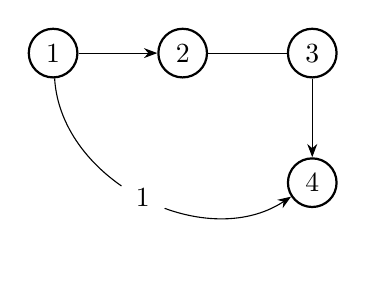
\begin{tikzpicture}
    \begin{scope}[every node/.style={circle,thick,draw}]
        \node(1){1};
        \node(2)[right=of 1] {2};
        \node(3)[right=of 2] {3};
        \node(4)[below=of 3] {4};
    \end{scope}
    %Lines
    \begin{scope}[>={Stealth[black]}, every node/.style={fill=white,circle}]
        \draw[-] (2.east) -- (3.west);
        \draw[->] (1.east) -- (2.west);
        \draw[->] (3.south) -- (4.north);
        \path [->] (1) edge[bend right=60] node {$1$} (4); 
    \end{scope}
\end{tikzpicture}

\subsection{Oppgaver}

\subsubsection{V2006 - Oppgave 6}
\textbf{a)} Er disse grafene isomorfe?
\begin{align*}
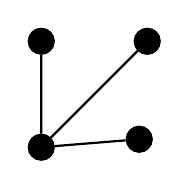
\begin{tikzpicture}
    \begin{scope}[every node/.style={shape=circle,draw, fill=black}]
        \node(1) {};
        \node(2)[right=of 1] {};
        \node(3)[below =of 1] {};
        \node(4)[below right = of 1] {};
    \end{scope}
    %Lines
    \draw[thick]   (1) -- (3)
            (3) -- (2)
            (3) -- (4); 
\end{tikzpicture}
\qquad
\qquad
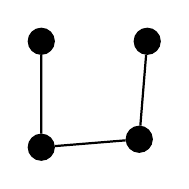
\begin{tikzpicture}
    \begin{scope}[every node/.style={shape=circle,draw, fill=black}]
        \node(1) {};
        \node(2)[right=of 1] {};
        \node(3)[below =of 1] {};
        \node(4)[below right = of 1] {};
    \end{scope}
    %Lines
    \draw[thick]   (1) -- (3)
            (4) -- (2)
            (3) -- (4); 
\end{tikzpicture}
\end{align*}

\noindent \textbf{b)} Finn 11 løkke-frie(loop-free) ikke-isomorfe uretta(non-directed) grafer med 4 hjørner.\\
\textbf{c)} Vis at de 11 grafene du fant i b) er alle mulige løkke-frie ikke-isomorfe uretta grafer med 4 hjørner.\\
\indent Tips: tell kanter.

\paragraph*{Løsning} %TODO

\newpage
\section{Formelle språk og endelige tilstandsmaskiner}

Formelle språk handler om alfabeter, og ord du kan danne med disse. Men her er \enquote{ord},
ikke helt det samme som det man forbinder med det i vårt vanlige språk, siden de ikke har noen betydnig.

Vi snakker ofte om et alfabet $\Sigma$, som er en mengde med bokstaver, for eksempel $\{0,1\}$, en streng
har dere sannsynligvis hørt om tidligere, og er en sammensetning med symboler. Vi har også $\lambda$ som er
en spesiell streng, som er tom. Med et alfabet, så kan du lage et språk, bare du lager regler for
hvilke ord du tillater.



\end{document}
